% Template for new reports written with the default style
% of LaTeX.
% 
% It relies on the existence of the files 'commands.tex'
% and 'bibl.bib' which are my constantly growing files
\documentclass{article}

\usepackage{amsfonts,amsmath}
\usepackage{graphicx,epsfig,psfrag}
%\usepackage{draftcopy}

% My usual user defined commands
% Bold letters
\newcommand{\bb}{\mathbf{b}}
\newcommand{\bc}{\mathbf{c}}
\newcommand{\be}{\mathbf{e}}
\newcommand{\bff}{\mathbf{f}}
\newcommand{\bm}{\mathbf{m}}
\newcommand{\bn}{\mathbf{n}}
\newcommand{\bt}{\mathbf{t}}
\newcommand{\bu}{\mathbf{u}}
\newcommand{\bx}{\mathbf{x}}
\newcommand{\by}{\mathbf{y}}
\newcommand{\bz}{\mathbf{z}}
\newcommand{\bX}{\mathbf{X}}
\newcommand{\bphi}{\boldsymbol{\phi}}

% Derivatives
\newcommand{\pdiff}[2]{\frac{\partial #1}{\partial #2}}
\newcommand{\diff}[2]{\frac{\mbox{d} #1}{\mbox{d} #2}}
\renewcommand{\div}{\mbox{div}\,}
\newcommand{\grad}{\mbox{grad}\,}
 
% Matrices
\newcommand{\vecTwo}[2]{\left( \begin{array}{c} #1 \\ #2 \end{array}\right)}
\newcommand{\vecThree}[3]{\left( \begin{array}{c} #1 \\ #2 \\ #3 \end{array}\right)}
\newcommand{\matrTwo}[4]{\left( \begin{array}{cc} #1 & #2 \\ #3 & #4 \end{array}\right)}
\newcommand{\matrThree}[9]{\left( \begin{array}{ccc} #1 & #2 & #3 \\ #4 & #5 & #6 \\ #7 & #8 & #9 \end{array} \right)}

%Miscellaneous
\newcommand{\myspace}{\hspace{0.5cm}}






\author{Carl Tro\"{e}ng \and Niklas Wikstr\"{o}m \and Mattias Liefvendahl}
\title{Mode-based fluid-structure interaction simulation}

\begin{document}

\maketitle

\section{Introduction} \label{sec:intro}

In this document we present a method for fluid-structure interaction (FSI) simulation
(see~\cite{DH:1} for a not very good review of the research area).
We describe both the theoretical formulation of the method, its implementation
and its verification for test problems.

The method relies on a modal description of the structure, which is performed
as a pre-processing step. Then the actual FSI-simulation is carred out in
an \texttt{OpenFOAM}-solver which includes functionality for the modal deformation
of the structure and its (time-resolved) coupling to the fluid motion.

The choice for structural solver for the initial test cases is \texttt{Comsol}.
This may be revised at a later stage of developments.

In section~\ref{sec:theory}, we describe the theory of the method,
in section~\ref{sec:impl}, we describe its implementation, and, in section~\ref{sec:tests},
we describe its verification for test cases.

\begin{figure}[htbp!]
\centering

\includegraphics[width=0.5\linewidth]{figures/dummy}
\caption{A dummy picture ...}
\end{figure}

\section{Theoretical formulation} \label{sec:theory}

We consider structures composed of an isotropic and homegeneous
elastic material. We assume that the deformations are sufficiently
small so that linear elasticity is a good approximation.
Furthermore, we typicall consider constant density, $\rho_s$,
and elasticity parameters.

We want to represent the motion of the structure by a relatively
small number of modes.
For this purpose, we perform a modal analysis of the structure, as a
pre-processing step before the FSI-problem is set up.
The output of the modal analysis is a set of $N$ modes and $N$ frequencies,
\[
\bphi_i(\bx),\,\,\omega_i,\hspace{1cm} i=1,\ldots,N.
\]
We use bold letters for vector quantities and normal font for scalar
quantities. The modes should be normalized using the density
of the solid in the following way.

\begin{equation}
\int_{V_s} \rho_s(\bx) |\bphi(\bx)|^2\,\mbox{d}V=1
\label{eq:volint}
\end{equation}

Here $V_S$ is the volume occupied by the structure (in the undeformed state),
and we note that the density typically is constant and can be ``moved
outside'' the integral.

Using the modes, we can represent the displacement, $\bu$, of the structure as,
\[
\bu(\bx,t)=\sum_{i=1}^N\alpha_i(t)\bphi_i(\bx),
\]
where we have introduced the time dependent mode coefficients, $\alpha_i$.

The fluid-structure coupling is obtained through the fluid forces on
the surface of the structure. In the initial stage we only include the
pressure forces, but at a later stage it may be useful to also include
the viscous forces. Thus each structural coefficient satisfies an ODE,
with a forcing term containing fluid forces.
\[
\frac{\mbox{d}^2\alpha_i}{\mbox{d}t^2}+
\omega_i^2\alpha_i=Q_i
\]
The forcing is given by the following expression.
\[
Q_i=-\int_S p\bn\cdot \bphi_i\,\mbox{d}S
\]
Here, $\bn$, is the local  unit normal of the surface pointing into the fluid.

\section{Implementation} \label{sec:impl}

The selection of implementation method is based on that the model should be
useful together
with any solver application supporting a dynamicFvMesh without changes to the
application. The application of the model should be specific to the OpenFOAM
case, not to the solver. Further, the user interface to the model should be
comprehendible, and not limited to a predefined number of modes.

Therefore the entire modal analysis model is implemented as a separate class,
that can be dynamically linked at runtime by the \texttt{libs ("library.so")}
directive in \texttt{system/controlDict}. Since the solid structure is
associated with fluid boundaries, the model is implemented as a boundary
condition and since the structural modes are associated with boundary
displacement, the boundary condition is a certain kind of point displacement
boundary condition.

\subsection{The modalDisplacement boundary condition}

The boundary condition serves to calculate and set point displacement vectors
for the patch points at each time step, based on fluid load and mode shapes
achieved from a modal analysis.

Thus, the following steps must be handled:

\begin{enumerate}
    \item Read mode shapes from modal analysis.
    \item If parallel: Distribute mode shapes to processors.
    \item Calculate the forcing term, $Q_i$ for each mode.
    \item Solve the ODE for mode coefficients, $\alpha_i$.
    \item Apply the resulting displacements to patch points.
\end{enumerate}

To achieve this, the boundary condition consists of two parts; The boundary
condition class itself, and an object handling the modes data and related calculations.
The boundary condition class constructs the structural modes,
when the boundary condition is constructed.

\subsubsection{The structuralModes class}

The class handling all modes calculations, is actually two classes: (1) A
\texttt{structuralMode} class, that manages reading and calculations of a
single mode and (2) a kind of a \texttt{List} class, \texttt{structuralModes},
that manages automatic construction of any number of \texttt{structuralMode}
objects, read from a dictionary and that has wrapper functions, calling
functions from each of its objects.  The implementation is borrowed from
e.g.~the implementation of porous zones.

The boundary condition, \texttt{modalDisplacement}, thus constructs its own
\texttt{structuralModes} list object, which in turn fills it self with all modes
defined in the associated dictionary. When the boundary condition is scheduled for
update (each time step), the boundary condition asks its structuralModes object
for the current point displacements and applies these.

\subsubsection{Parallelisation}

A mode shape from the modal analysis, needed to create a
\texttt{structuralMode}, consists of a list of vectors. Each vector in the list
corresponds to the displacement of a point in the moving patch and the vector list
has the same length as the number of points in the corresponding patch.
Specifically, the vector list corresponds to the the points of the patch in the
\emph{serical} case. Therefore, for parallel runs, the mode information must be
carefully distributed to each process. This is managed by the boundary condition,
which includes tables and functions that maps serial point labels to parallel
counterparts and vice versa.

To enable the construction of the label maps, the pre-processing step must include
generation of a file, containg a list of the serial case patch point labels.
An application is written to create this file.



\subsection{Usage of the modalDisplacement boundary condition}

First of all, a solver that implements a \texttt{dynamicFvMesh} is needed.
E.g.~pimpleDyMFoam or interDyMFoam. The dynamicFvMesh requires two case files:

\begin{itemize}
    \item A point field, \texttt{pointDisplacement}.
    \item A dictionary, \texttt{constant/dynamicMeshDict}, defining the
          motion solver to be used (standard to dynamic mesh codes).
\end{itemize}

Both of the above are commonly found in the tutorials and are not specific to the
modalDisplacement boundary condition.

Secondly, and unique to the present implementation, is the dicitonaries and
boundary condition definition needed for the modalDisplacement boundary
condition. The dictionaries are all stored in the directory
\texttt{constant/structuralModes/}, and consist of the following:

\begin{itemize}
    \item \texttt{fluidProperties}: Defines fluid density, since the solver might be incompressible.
    \item \texttt{modeData\_<patchName>}: Contains definition of each structural mode.
    \item \texttt{labels\_<patchName>}: A list of the serial point labels for the patch. This file is
        generated by the \texttt{writePatchPointLabels} utility.
    \item \texttt{monitorPoints\_<patchName>}: An optional list of point coordinates, which
        displacements are reported on standard output.
\end{itemize}

The \texttt{modeData\_\ldots} dictionary consists of a list of sub-dictionaries. Each describing
one structural mode. For a simulation including two modes only, it has the following form (excluding the header):

\begin{verbatim}
...
2
(
    first
    {
        generateMode no;
        frequency     10;
        scalingFactor 1;
        modeDisplacement
        #include "firstModeDisplacements.dat"
    }

    second
    {
        generateMode yes;
        generatedMode
        {
            origin  (0 0 0);
            axis    (0 0 1);
            waveLength   0.5;
            amplitude (0.05 0 0);
        }

        frequency     25;
        scalingFactor 1;
        modeDisplacement 0();
    }
)
\end{verbatim}

The first mode shape is based on existing data residing in the file \texttt{firstModeDisplacements.dat}.
This data file contains a vectorField with displacements corresponding to the patch points. The second
mode examplifies the posibility to let the boundary condition generate a mode. Presently this mode is
a simple trigonometric function, suitable for beams.

\section{Test cases} \label{sec:tests}

The following is a tentative list of test cases for the algorithm.
\begin{enumerate}
\item A moving box in a fixed pressure field. No FSI, but testing
of several components in the program.
\item A beam mounted perpendicular to the flow. The beam is fixed to
the floor at one end and free to move at the other.
\item An elastic hydrofoil with varying angle of attack, \cite{DY:1}.
\item A propeller blade in a varying inflow.
\item A hull structure excited by non-steady propulsion force.
\end{enumerate}

The beam test case is fundamental for the verification of the
algorithm and the implementation, and several tests should be
performed for the beam. Apart from cross-flow, the beam should
be tested in a still fluid, to check the change in oscillation
frequency due to the added mass of the surrounding fluid.
When started in cross-flow, the beam should first bend in the flow
direction and then, when vortex shedding starts, it should go
over to oscillations in the transversal direction.

%--------------------------------------------
%
%     M O V I N G   B O X
%
\subsection{The moving box}

This test case does not contain fluid-structure interaction but
is designed to only check the following parts of the implementation.
\begin{itemize}
\item Input and output concerning the structural mode description.
\item Construction of the right hand side in the ODE for the mode coefficients.
\item Solution of the ODE for the mode coefficients.
\end{itemize}

The geometry is a rectangular box inside a cube.
The sides of the boxes are aligned with the coordinate directions.
The outer box is stationary and the inner
box can move as a rigid body along the coordinate axes.
The geometrical parameters of the problem are given in table~\ref{tab:boxParam}.
The motion of the body is driven by a prescribed pressure field which is contant
in time and is given by the expression,
\[
p=\left\{\begin{array}{lll}
\Delta p & \mbox{for} & x>0.5 \\
0 & \mbox{for} & x \leq 0.5
\end{array}\right.
\]
The pressure jump, $\Delta p$, and other physical parameters are given in
table~\ref{tab:boxPar}, and the pressure distribution is illustrated in 
figure~\ref{fig:boxP}.

\begin{figure}
\centering
\caption{The pressure distribution for the moving box test case, on the plane~$z=0$.}
\label{fig:boxP}
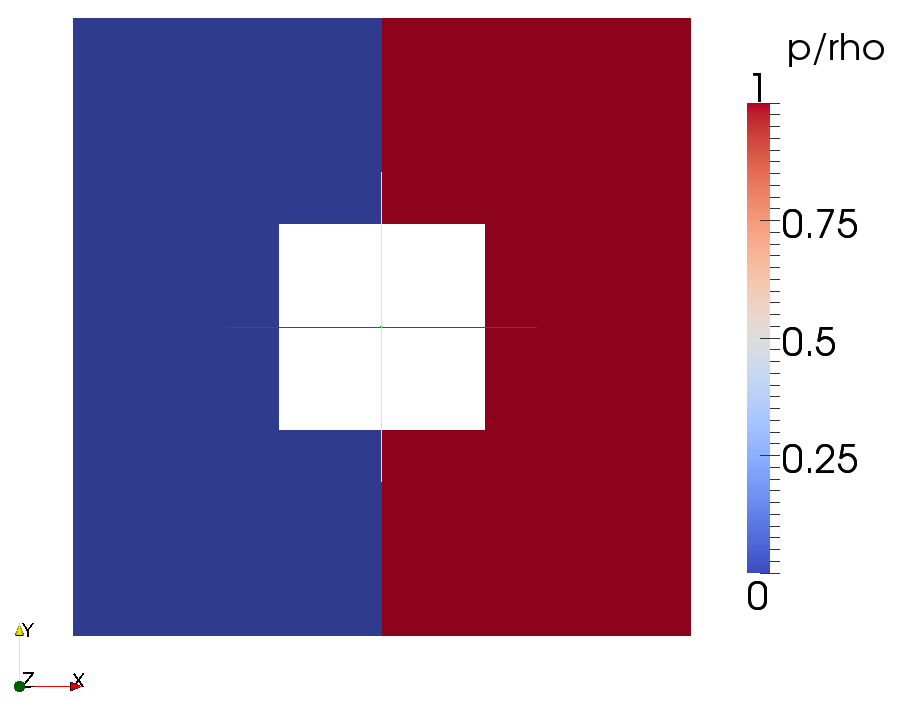
\includegraphics[width=0.7\linewidth]{figures/ml/fig1}
\end{figure}


\begin{table}[htp!]
\centering
\caption{The dimensions of the outer and inner boxes. All quantities
are given in meters, square meters or cubic meters as appropriate.}
\label{tab:boxParam}
\begin{tabular}{c|cc|}
&  Outer box & Inner box  \\ \hline
$x_{min}$ & 0  & $1/3\approx 0.3333$  \\
$x_{max}$ & 1  & $2/3\approx 0.6667$  \\
$y_{min}$ & 0  & $1/3\approx 0.3333$  \\
$y_{max}$ & 1  & $2/3\approx 0.6667$  \\
$z_{min}$ & 0  & $3/7\approx 0.4286$  \\
$z_{max}$ & 1  & $4/7\approx 0.5714$  \\ \hline 
$V$  & 1 & $1/63\approx 0.0159$ \\
$A_x=A_y$ & 1 & $1/21\approx 0.0476$ \\
$A_z$ & 1 & $1/9\approx 0.1111$ \\  \hline
\end{tabular}
\end{table}

\begin{table}[htp!]
\centering
\caption{Physical parameters. Note that the solid density can be calculated
from the prescribed modal functions, as described in the text.}
\label{tab:boxPar}
\begin{tabular}{l|ccc|}
Quantity & Notation & Value & Unit \\ \hline
Fluid density & $\rho_f$ & 1000 & kg/m$^3$ \\
Pressure jump & $\Delta p$ & 1000 & Pa \\ \hline
\end{tabular}
\end{table}


The modal motion of the box is represented by three modes with the
frequencies,
\[
f_1=1\,\mbox{Hz},\hspace{1cm}
f_2=2\,\mbox{Hz},\hspace{1cm}
f_3=3\,\mbox{Hz},
\]
and mode shapes corresponding to rigid body motion in the three coordinate directions,
\[
\bphi_1(\bx)=a \be_x\hspace{1cm}
\bphi_2(\bx)=a \be_y\hspace{1cm}
\bphi_3(\bx)=a \be_z,
\]
where, $a=0.1\,$m.


The only way that the solid density enters the algorithm is through the normalization
of the modes. Given the information above, we can thus calculate which structural
density, $\rho_s$, it corresponds to.
\[
1=\int_{V_s}\rho_s|\bphi(\bx)|^2\,\mbox{d}V=\rho_s V_i\cdot a^{2}
\]
Using this expression and the inner box volume given in table~\ref{tab:boxParam},
we obtain, $\rho_s=6300\,$kg/m$^3$.

For this case, the forcing integrals can be evaluated analytically. For the first mode,
we have,
\[
Q_1=-\int_S p\bn\cdot \bphi_i\,\mbox{d}S=-\Delta p A_x a \approx -4.76 \mbox{Nm}.
\]
For the second and third modes, the forcing is zero, $Q_2=Q_3=0$.

\subsubsection{Analytical solution of first mode motion}

The motion of the block can thus be calculated by the solution of the ODE
for the first mode coefficient,
\[
\frac{\mbox{d}^2\alpha_1}{\mbox{d}t^2}+
\omega_1^2\alpha_1=Q_1,
\]
with inital data,
\[
\alpha_1(0)=0, \hspace{1cm} \dot{\alpha}(0)=0.
\]
The solution is given by the following convolution expression, for a general
time dependent forcing $Q_1(t)$, which then can be simplified since in the present case,
the forcing is constant.
\[
\alpha_1(t)=\frac{1}{\omega_1}\int_0^t \sin\left[
\omega_1(t-\tau)
\right] Q_1(\tau)\,\mbox{d}\tau=
\frac{Q_1}{\omega_1^2}(1-\cos \omega_1t)
\]

\subsubsection{Computed motion of the first mode}

The problem is solved by a program which involves all the functionality related to
the structural motion, but without the fluid solver. As described above, only
a pressure field (constant in time) is provided, which drives the structural motion.
Now we describe how input is provided to the program.

\vspace{0.2cm}

\noindent 1. The modes are described in the file:

\texttt{constant/structuralModes/modeData\_movingBlock}

\noindent Here is a segment of this input file relating to the first mode:

------------------------------

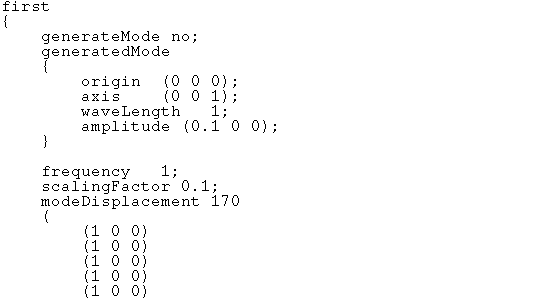
\includegraphics[width=0.7\linewidth]{figures/ml/data1}

------------------------------

\vspace{0.2cm}

\noindent 2. The input to the mesh deformation is given in the file:

\texttt{constant/dynamicMeshDict}

\noindent This file contains the following information:

------------------------------

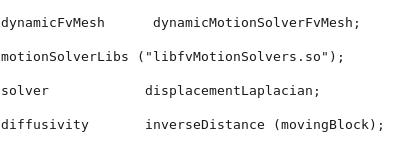
\includegraphics[width=0.55\linewidth]{figures/ml/data2}

------------------------------

\vspace{0.2cm}

\noindent 3. The remaining input, initial grid, pressure field, controls for time stepping etc,
are given in the same way as for a standard simulation case.
The case is simulated on the time interval, $0<t<10\,\mbox{s}$, with a time
step, $\Delta t = 0.01\,\mbox{s}$.

\begin{figure}[htbp!]
\centering
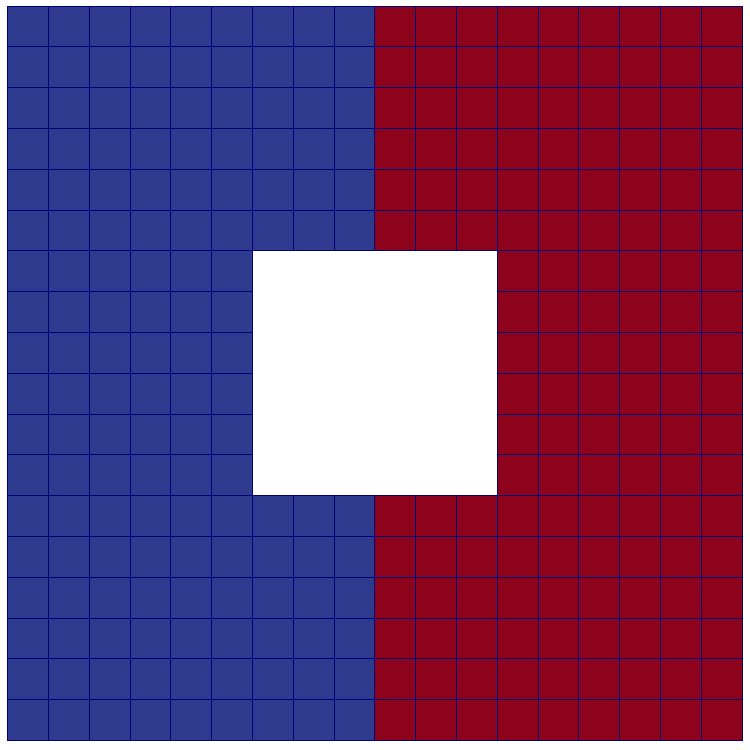
\includegraphics[width=0.4\linewidth]{figures/ml/noDef}
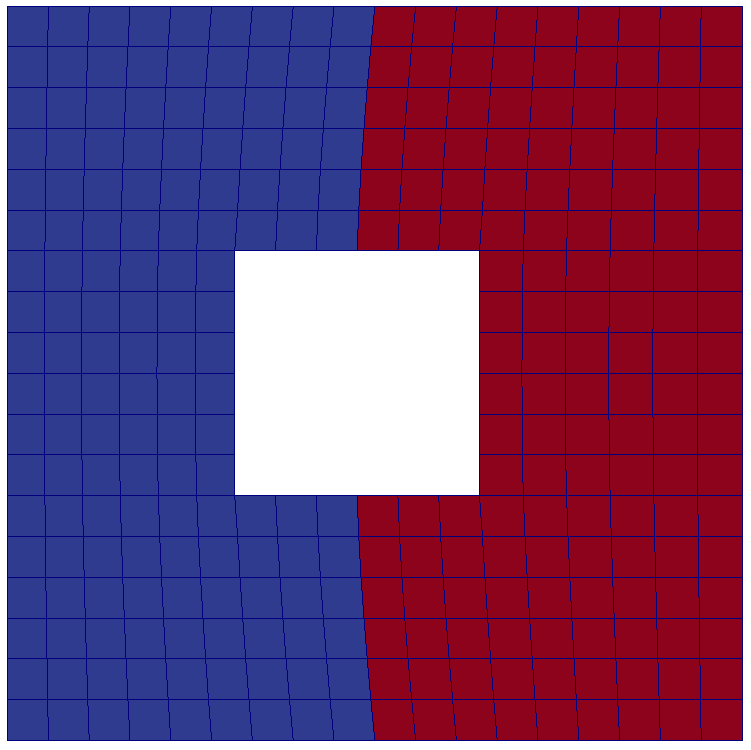
\includegraphics[width=0.4\linewidth]{figures/ml/maxDef}
\caption{Initial (undeformed) stat to the left, and maximal displacement, at $t=0.5\,$s,
to the right.}
\label{fig:boxDef}
\end{figure}

In figure~\ref{fig:boxDef}, we illustrate the grid deformation in the most deformed
state, at $t=0.5\,$s, and compare it to the initial grid.

\begin{figure}[htbp!]
\centering
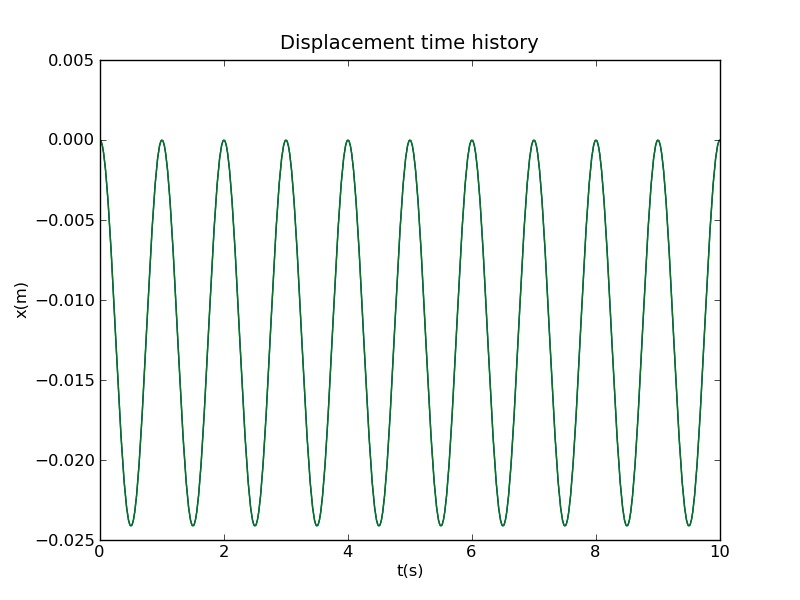
\includegraphics[width=0.49\linewidth]{figures/ml/displ.jpg}
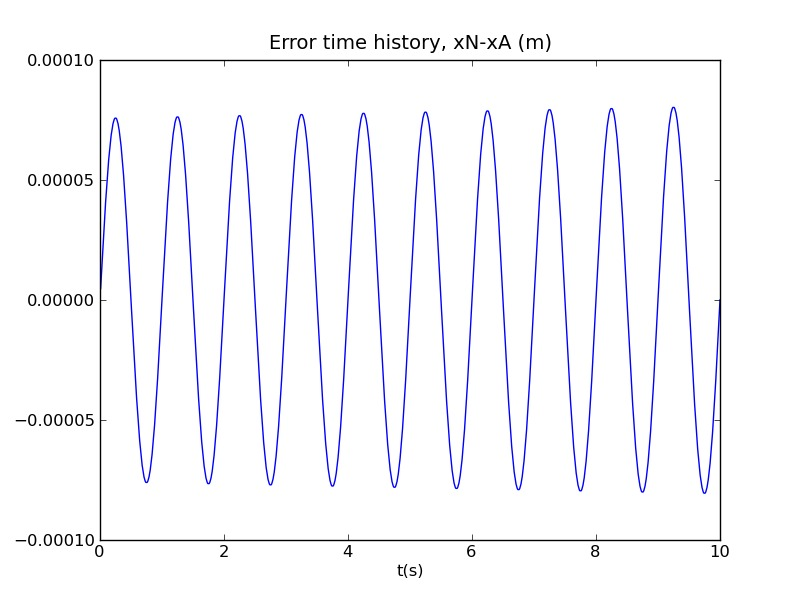
\includegraphics[width=0.49\linewidth]{figures/ml/diff.jpg}
\caption{Box displacement (in $x$-direction)
as function of time, $x_N(t)$, to the left, and error, $x_N(t)-x_A(t)$, to the right.}
\label{fig:displ}
\end{figure}

In order to check the computed motion, we post-process the computed displacement
for a point on the box. The displacement is only in the $x$-direction, and we
denote it by $x_N(t)$, where the sub-script indicates ``numerical''. We also
compare this to the exact analytical solution for the displacement, which we
denote $x_A(t)$. The displacement and the error are shown in figure~\ref{fig:displ}.
We note that the error is less than 0.34\% of the oscillation amplitude
over the whole simulation interval.

\subsection{The beam}

Cantilever beam = fixed at one end ...

The material parameters seem to correspond to something like rubber ...

\begin{table}[htbp!]
\centering
\caption{Material and geometrical parameters of the cantilever beam
with quadratic cross section and cross-sectional area $D^2$.}
\begin{tabular}{l|ccc|}
Quantity & Notation & Value & Unit \\ \hline
Modulus of elasticiy & $E$ & 0.03 & GPa \\
Poisson's ratio & $\nu_s$ & 0.3 & - - - \\
Density & $\rho_s$ & 5000 & kg/m$^3$ \\ \hline
Length & $L$ & 0.1 & m \\
Width & $D$ & 0.02 & m \\ \hline
\end{tabular}
\end{table}

\subsubsection{Mode generation, interpolation to CFD and scaling}

Two modal analyses are performed in two softwares. Comsol Multiphysics and
Ansys.  Both softwares delivered the same mode shapes, but the mode
normalisation was only successfully made in Ansys. The latter has as default
normalisation option to scale the modes with the \emph{mass matrix}, which
turns out to comply with the above equation \ref{eq:volint}, as discussed
below.

Mode data are exported from the structural solver as displacement vectors at
each solid mesh point, in ascii column data file format, where each row
contains point coordinates and corresponding displacement. This data then be
interpolated to the CFD boundary using the implemented OpenFOAM utility
\texttt{interpolateModeData}. In short, this utility reads a set of "mode
files" exported from the structural solver, and writes their interpolated
counterparts to another set of files. The latter is then included in the
dictionary defining the modes to be included in the OpenFOAM FSI.

To be able to assert that each mode fulfills equation \ref{eq:volint},
another utility is written: \texttt{calculateModeScaleFactor}. This
utility requires the same dictionary input as the FSI case, but must
be run on the solid itself. That is, a mesh in the solid region needs
to be generated. In the case of the cantilever beam, this is trivial.

When mode data for the first five modes from Ansys are interpolated to the
OpenFOAM case consisting of the solid beam, \texttt{calculateModeScaleFactor}
is run on each of the modes and the result is assuring: For all bending modes
the scale factor calculated by the OpenFOAM utility is very close to unity.
The exception is the third torsion mode, for which the scale factor seem to
be more difficult to calculate based on displacements in a cartesian system.

To conclude: Modes exported from a structural solver can be interpolated
to the OpenFOAM case and in case the normalisation of these modes is believed
to disagree with equation \ref{eq:volint}, the scale factor can be calculated
using an OpenFOAM case consisting of the solid only.


\bibliography{bibl/ml,bibl/nw,bibl/ct}
\bibliographystyle{plain}

\end{document}
